\subsection{Связь между суммами и интегралами. Интегральный признак. Сходимость и расходимость рядов $\sum \frac{1}{n^p}$ и $\sum \frac{1}{n \ln n}$}
\begin{theorem} (связь между суммами и интегралами)

    \quad Пусть $f: [a, b] \to \R$ монотонна. Тогда \[ \left| \sum_{k = a}^b f(k) - \int_a^b f(x)dx \right| \leqslant \max\{|f(a)|, |f(b)| \}\] 
\end{theorem}
\begin{proof}
    Пусть $f$ монотонно убывает и $f \geqslant 0$.
    Посмотрим на 2 суммы: \[ \sum\limits_{k = a}^{b-1} f(k) \geqslant \int_a^b f(x)dx \geqslant \sum\limits_{k = a + 1}^b f(k) \]
    \begin{center}
        %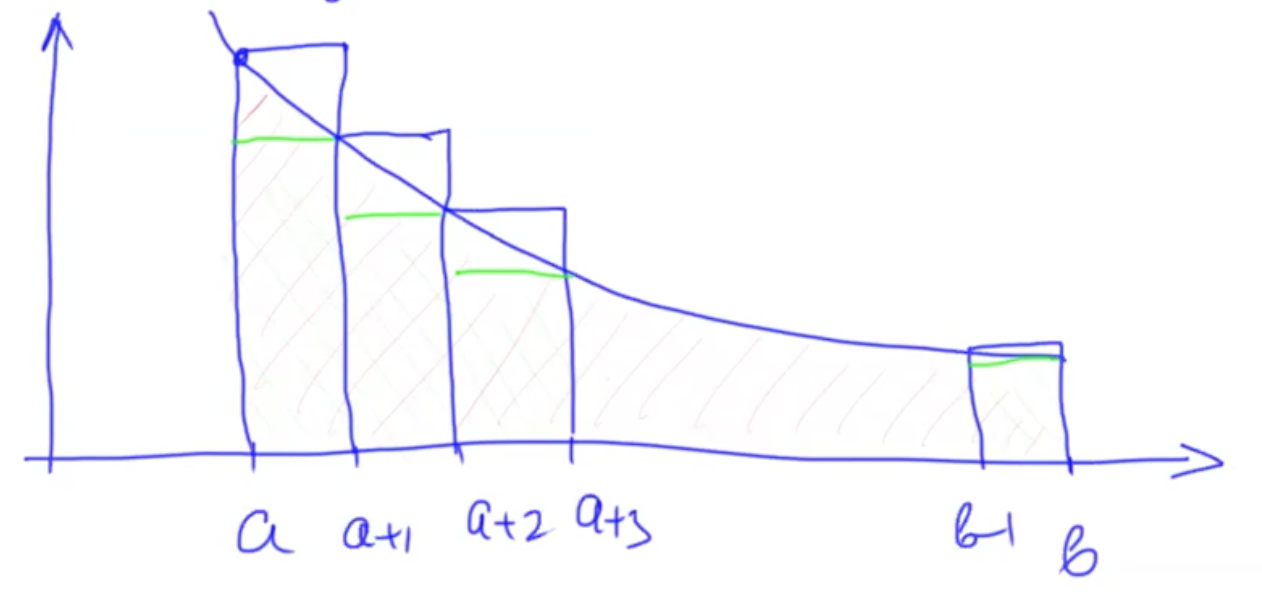
\includegraphics[scale=0.5]{images/lec5_pic1.png}
        \begin{tikzpicture}[thick,yscale=0.8]
            % Axes
            \draw[-latex,name path=xaxis] (-1,0) -- (10,0) node[above]{};
            \draw[-latex] (0,-2) -- (0,8) node[right]{};
            
            % Function plot
            \draw[ultra thick, orange,name path=function]  plot[smooth,domain=1.2:8] (\x, {1/(0.2*\x-0.1) + 0.6}) node{};

            % Draw columns
            \draw[ultra thick, violet, name path=0function] (1.5, 0) -- (1.5, 5.5) node[circle,fill,inner sep=1pt]{};
            \draw[ultra thick, violet, name path=1function] (2.5, 0) -- (2.5, 5.5);
            \draw[ultra thick, violet] (1.5, 5.5) -- (2.528, 5.5);

            \draw [ultra thick, pink, name intersections={of=function and 1function}] ($(intersection-1)+(0.028,0)$) -- ++(-1,0);
            \draw [ultra thick, violet, name intersections={of=function and 1function}] ($(intersection-1)-(0.028,0)$) -- ++(1.056,0);
            \draw [ultra thick, violet, name intersections={of=function and 1function}, name path=2function] ($(intersection-1)+(1,0)$) -- ++(0,-3.1);

            \draw [ultra thick, pink, name intersections={of=function and 2function}] ($(intersection-1)+(0.028,0)$) -- ++(-1,0);
            \draw [ultra thick, violet, name intersections={of=function and 2function}] ($(intersection-1)-(0.028,0)$) -- ++(1.056,0);
            \draw [ultra thick, violet, name intersections={of=function and 2function}, name path=3function] ($(intersection-1)+(1,0)$) -- ++(0,-2.26);

            \draw [ultra thick, pink, name intersections={of=function and 3function}] ($(intersection-1)-(0.028,0)$) -- ++(-0.944,0);

            \draw[ultra thick, violet, name path=5function] (7, 0) -- (7, 1.4);
            \draw[ultra thick, violet, name path=4function] (8, 0) -- (8, 1.4);
            \draw[ultra thick, violet] (6.972, 1.4) -- (8.028, 1.4);
            \draw[ultra thick, pink] (7.028, 1.25) -- (7.972, 1.25);
            
            % % x-axis labels
            \draw [name intersections={of=0function and xaxis}] ($(intersection-1)+(0,0.1)$) -- ++(0,-0.2) node[below] {\small $a$} ;
            \draw [name intersections={of=1function and xaxis}] ($(intersection-1)+(0,0.1)$) -- ++(0,-0.2) node[below] {\small $a+1$} ;
            \draw [name intersections={of=2function and xaxis}] ($(intersection-1)+(0,0.1)$) -- ++(0,-0.2) node[below] {\small $a+2$} ;
            \draw [name intersections={of=3function and xaxis}] ($(intersection-1)+(1,0.1)$) -- ++(0,-0.2) node[below] {\small $a+3$} ;
            \draw [name intersections={of=5function and xaxis}] ($(intersection-1)+(0,0.1)$) -- ++(0,-0.2) node[below] {\small $b-1$} ;
            \draw [name intersections={of=4function and xaxis}] ($(intersection-1)+(0,0.1)$) -- ++(0,-0.2) node[below] {\small $b$} ;
        \end{tikzpicture}
    \end{center}
    \quad Случай, когда $f$ не обязательно неотрицательна, сводится к этому прибавлением константы.
    Действительно, сделаем функцию неотрицательной прибавлением константы $c$, тогда как суммы, так и интеграл изменятся на $+c(b - a)$, то есть неравенство сохранится.

    \quad Теперь вычтем из неравенства всю сумму: \[ -f(b) \geqslant \int_a^b f(x)dx - \sum\limits_{k = a}^b f(k) \geqslant -f(a) \]
    \quad Добавив модуль, получаем искомое неравенство.

    \quad Случай, когда $f$ монотонно возрастает рассматривается аналогично.
\end{proof}

\vspace{6mm}

\textbf{Интегральный признак.}
Пусть $f: [1, +\infty) \to [0, +\infty)$ монотонна. 
Тогда $\sum\limits_{n = 1}^\infty f(n)$ и $\int_1^{+\infty} f(x)dx$ ведут себя одинаково. 
\begin{proof}
    Если $f$ монотонно возрастает, то, очевидно, и то, и то расходится.
    Пусть $f$ монотонно убывает. 
    Члены ряда неотрицательны, поэтому его сходимость равносильна ограниченности частичных сумм $S_n := \sum\limits_{k = 1}^n f(k)$.
    Сходимость же интеграла равносильна ограниченности первообразной $F(x) := \int_1^x f(x)dx$.  
    Чтобы связать эти ограниченности воспользуемся теоремой: \[ \left| S_n - F(n) \right| \leqslant f(1) (\text{не рассматриваем $f(n)$ так как $f$ убывает}) \]
    \quad Значит, ограниченность $S_n \Leftrightarrow$ ограниченность $F(n)$.
    
    \quad Но мы брали первообразную только в натуральных точках, значит, нам надо еще понять, что ограниченность $F(n) \Leftrightarrow$ ограниченность $F(x)$.
    Это очевидно, так как из-за неотрицательности $f$ первообразная $F$ монотонно возрастает, а значит, $F(x) \leqslant F(n)$ при $x \leqslant n$.

    \quad Таким образом, мы показали, что ограниченность $S_n \Leftrightarrow$ ограниченность $F(x)$. 
    Следовательно, мы показали равносильность сходимости суммы и интеграла.
\end{proof}

\vspace{6mm}

\begin{example}
    Установим, при каких $p$ сходится ряд $\sum\limits_{n = 1}^{\infty} \frac{1}{n^p}$.
    При $p \leqslant 0$, ряд очевидно расходится. 
    Пусть $p > 0$.
    Введем функцию $f(x) = \frac{1}{x^p}$, которая неотрицательна и монотонно убывает. 
    Тогда согласно интегральному признаку $\sum\limits_{n = 1}^{\infty} \frac{1}{n^p}$ и $\int_1^{+\infty} \frac{dx}{x^p}$ ведут себя одинаково. 
    А про интеграл мы уже все знаем, он сходится, когда $p > 1$. 
    Следовательно, $\sum\limits_{n = 1}^{\infty} \frac{1}{n^p}$ сходится при $p > 1$.
\end{example}

\begin{follow}
    С таким рядом удобно писать признак сравнения: если $0 \leqslant a_n \leqslant \frac{c}{n^p}$ при $p > 1$, то $\sum a_n$ сходится. 
\end{follow}

\begin{example}
    Исследуем на сходимость ряд $\sum\limits_{n = 2}^\infty \frac{1}{n\ln n}$. 
    Введем функцию $f(x) = \frac{1}{x\ln x}$. Она $> 0$ и монотонно убывает $\Rightarrow$ интегральный признак: \[ \int_2^{+\infty} \frac{dx}{x\ln x} = \ln(\ln x)\big|_2^{+\infty} = +\infty \]
    Значит, ряд расходится. 
\end{example}

